\documentclass[11pt]{article}
\usepackage[margin=0.9in]{geometry}
\usepackage[T1]{fontenc}
\usepackage{lmodern,microtype}
\DisableLigatures[-]{family=tt*}   % keep "--" as two hyphens in command-line options
\usepackage{float}
\usepackage{amsmath}
\usepackage{graphicx,booktabs,tabularx,array}
\usepackage{enumitem}
\usepackage[dvipsnames]{xcolor}
\usepackage{fancyvrb}
\usepackage[font=small,labelfont=bf]{caption}
\usepackage{subcaption}
\usepackage{tikz}
\usetikzlibrary{arrows.meta,positioning,calc,fit,backgrounds}
\usepackage[most]{tcolorbox}
\usepackage{hyperref}
\usepackage[capitalise]{cleveref}

\hypersetup{colorlinks=true,linkcolor=NavyBlue,urlcolor=NavyBlue}
\setlist{itemsep=2pt,topsep=4pt}
\graphicspath{{figures/}}

% file / command names with underscores etc.
\newcommand{\file}[1]{\texttt{\detokenize{#1}}}
\newcommand{\key}[1]{\tikz[baseline=(k.base)]\node[draw,rounded corners=2pt,inner sep=2pt,font=\ttfamily\footnotesize](k){#1};}

% terminal commands
\DefineVerbatimEnvironment{cmd}{Verbatim}{fontsize=\small,frame=single,framesep=2mm,
  rulecolor=\color{gray!60},formatcom=\color{black!85}}

\newtcolorbox{note}[1][Note]{colback=yellow!6,colframe=orange!70!black,fonttitle=\bfseries,
  title=#1,left=2mm,right=2mm,top=1mm,bottom=1mm}
\newtcolorbox{say}{colback=NavyBlue!4,colframe=NavyBlue!70,fonttitle=\bfseries,
  title=What to say,left=2mm,right=2mm,top=1mm,bottom=1mm}

\tikzset{
  box/.style={draw,rounded corners=3pt,align=center,inner sep=5pt,font=\small,fill=white},
  arr/.style={-{Stealth[length=2.5mm]},thick},
}

\title{\textbf{gr00t-arm}\\[2pt]\large A desk robot arm that learns from demonstrations with NVIDIA GR00T\\[2pt]
\normalsize How it connects to GR00T, and how to build, wire, calibrate, train and run it}
\author{Yishane Kao\\[2pt]\small Arm: \emph{Easy Robot Arm} by mobiobi
  (\href{https://www.printables.com/model/97370}{Printables 97370}), CC BY-NC-SA, used unmodified}
\date{October 2026}

\begin{document}
\maketitle
\tableofcontents
\clearpage

%======================================================================
\part{How the arm connects to GR00T}
%======================================================================

\section{The idea in one picture}

GR00T is NVIDIA's \emph{robot foundation model}: one neural network, pretrained on a huge
amount of robot and human data, that turns \textbf{what a robot sees}, \textbf{what it is
told} and \textbf{where its joints are} into \textbf{the next motions}. It was built for
humanoids, but it is designed so a \emph{new} body can be taught to it with a small amount of
data. This arm is that new body: five \$2 servos, a webcam for eyes, and 100--200
demonstrations. A ball and a block sit on the plate; you type ``pick up the ball'' or ``pick up
the block'', and the arm drops that one in the cup. The words decide which object it goes for.

\begin{figure}[htbp]
\centering
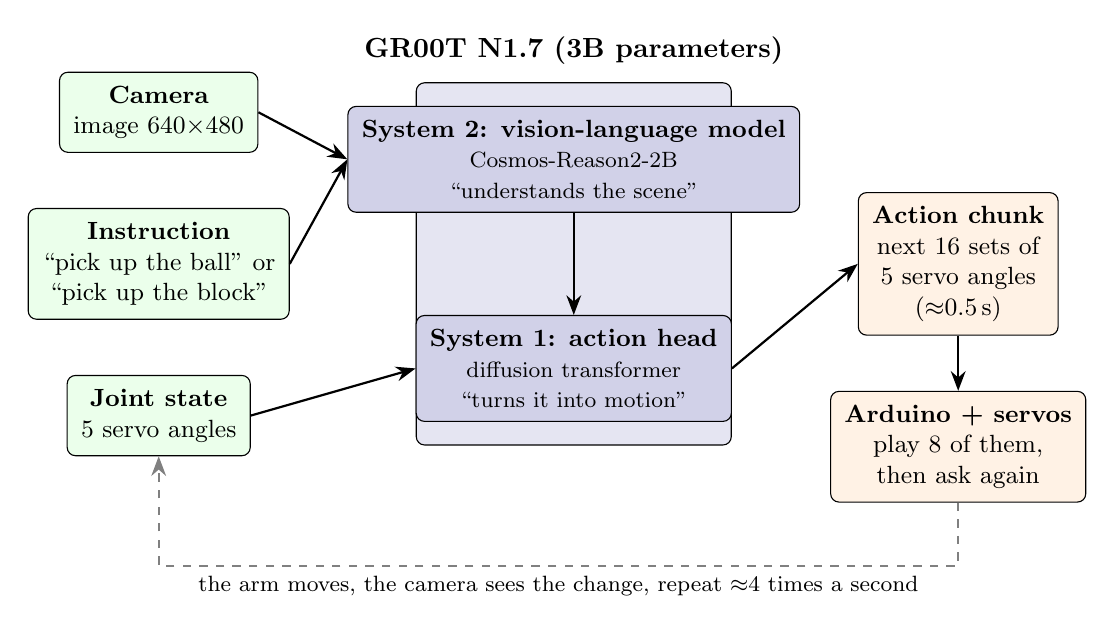
\begin{tikzpicture}[node distance=7mm and 9mm]
  \node[box,fill=green!8] (cam) {\textbf{Camera}\\ image $640{\times}480$};
  \node[box,fill=green!8,below=of cam] (lang) {\textbf{Instruction}\\ ``pick up the ball'' or\\ ``pick up the block''};
  \node[box,fill=green!8,below=of lang] (state) {\textbf{Joint state}\\ 5 servo angles};

  \node[box,fill=NavyBlue!10,right=16mm of lang,minimum width=40mm,minimum height=46mm] (g) {};
  \node[box,anchor=north,fill=NavyBlue!18] (vlm) at ($(g.north)+(0,-3mm)$)
     {\textbf{System 2: vision-language model}\\ \footnotesize Cosmos-Reason2-2B\\ \footnotesize ``understands the scene''};
  \node[box,anchor=south,fill=NavyBlue!18] (dit) at ($(g.south)+(0,3mm)$)
     {\textbf{System 1: action head}\\ \footnotesize diffusion transformer\\ \footnotesize ``turns it into motion''};
  \node[font=\bfseries,above=1mm of g] {GR00T N1.7 (3B parameters)};
  \draw[arr] (vlm) -- (dit);

  \node[box,fill=orange!10,right=16mm of g] (chunk) {\textbf{Action chunk}\\ next 16 sets of\\ 5 servo angles\\ ($\approx$0.5\,s)};
  \node[box,fill=orange!10,below=of chunk] (arm) {\textbf{Arduino + servos}\\ play 8 of them,\\ then ask again};

  \draw[arr] (cam.east) -- (vlm.west);
  \draw[arr] (lang.east) -- (vlm.west);
  \draw[arr] (state.east) -- (dit.west);
  \draw[arr] (dit.east) -- (chunk.west);
  \draw[arr] (chunk) -- (arm);
  \draw[arr,dashed,gray] (arm.south) |- ++(0,-8mm) -| (state.south)
     node[pos=0.25,below,font=\footnotesize,black]{the arm moves, the camera sees the change, repeat $\approx$4 times a second};
\end{tikzpicture}
\caption{The control loop. Everything on the left is produced by this arm; the middle is GR00T; the right is sent back to the arm.}
\label{fig:loop}
\end{figure}

\section{What GR00T is, in plain words}

\begin{description}[leftmargin=0pt]
\item[A foundation model for robots.] Language models are pretrained on the internet and then
  adapted to a task. GR00T does the same for robot \emph{motion}: it is pretrained on a mix of
  real robot recordings, simulated robots and videos of humans, then \emph{post-trained}
  (fine-tuned) on a small set of demonstrations of a specific robot doing a specific task
  \cite{gr00tn1,isaacgr00t}.
\item[Two systems, like fast and slow thinking.] The \textbf{System 2} part is a
  vision-language model: it looks at the camera image and reads the instruction, and turns
  them into \emph{embeddings}: long lists of numbers that capture what is in the scene and what
  was asked. Not words, and not positions. The \textbf{System 1} part is the \emph{action
  head}, a diffusion transformer: it takes those numbers plus the robot's current joint angles
  and generates the motor commands itself. System 2 is the ``what is going on and what should
  happen'', System 1 is the ``how do my joints get there''.
\item[It learns by copying, not by trial and error.] Fine-tuning shows GR00T the recorded
  demonstrations and trains it to output what the demonstration did next in each situation
  (\emph{imitation learning}). There is no reward and no practising on the real arm. It never
  gets told where the ball is: it works that out from the camera image, which is the part the
  AI is for.
\item[It outputs a short plan, not one move.] The action head predicts an \textbf{action
  chunk}: the next 16 commands (about half a second). Predicting a chunk makes motions smooth
  and lets the model commit to a plan instead of dithering every frame. We play the first 8 and
  then ask again with a fresh image, so the arm keeps correcting itself.
\item[How it generates actions: denoising.] The action head starts from random numbers and
  refines them over a few steps (4 by default) into a sensible chunk, guided by what System 2
  saw. This ``flow matching'' / diffusion trick is the same family of method image generators
  use, applied to joint angles instead of pixels.
\item[One brain, many bodies.] The big shared network is the same for every robot. What is
  specific to a body is small: how its joint state is read in and how actions are read out.
  GR00T has a reserved slot for robots it has never seen, \texttt{NEW\_EMBODIMENT}. Our arm is
  registered there with 4 arm joints, 1 gripper and 1 camera.
\end{description}

\section{Every GR00T concept, and where it lives on this arm}

\begin{table}[htbp]
\centering\small
\caption{Mapping GR00T's pieces onto the arm. File names are in the GitHub repo.}
\label{tab:map}
\begin{tabularx}{\linewidth}{@{}>{\raggedright}p{3.0cm}>{\raggedright}X >{\raggedright\arraybackslash}p{3.9cm}@{}}
\toprule
GR00T concept & On this arm & Where \\
\midrule
Vision input & One USB webcam on a fixed mast looking down at the work area (key \texttt{front}). Fixed so every demo looks the same. & mast + webcam mount, \file{arm_io.py} \\
Language instruction & ``pick up the ball'' or ``pick up the block'', saved with each demo; typed in at run time & \file{recorder.py}, \file{run_policy.py} \\
Proprioceptive state & 5 servo angles in degrees: base, shoulder, elbow, wrist (\texttt{single\_arm}) and gripper (\texttt{gripper}) & \file{export_dataset.py} \\
Embodiment & \texttt{NEW\_EMBODIMENT} with our modality config & \file{gr00t_arm_config.py} \\
Dataset format & LeRobot v2.1 + \file{meta/modality.json} (parquet tables + mp4 videos) & \file{export_dataset.py} \\
Action chunk & 16 future commands; we execute 8 then re-query & \file{run_policy.py} \\
Relative vs absolute actions & Arm joints are predicted as \emph{changes} from the current angles (generalises better); the gripper as an absolute open/close target & \file{gr00t_arm_config.py} \\
Post-training & Fine-tune on 100--200 demos on a rented cloud GPU, $\approx$3000 steps & \file{gr00t/finetune.sh} \\
Inference & Model runs on the cloud GPU as a server; the laptop sends image + state, gets actions back over ZeroMQ & \file{gr00t/serve.sh}, \file{policy_client.py} \\
Demonstrations & Scripted pick-and-place (auto-collected; random layout, ball or block about half each) or keyboard teleop & \file{autodemo.py}, \file{teleop.py} \\
Simulation data & A MuJoCo copy of the arm records extra demos at varied positions and scores models automatically; GR00T's pretraining also mixes in simulated robots & \file{sim.py} \\
\bottomrule
\end{tabularx}
\end{table}

\section{The whole pipeline}

\begin{figure}[htbp]
\centering
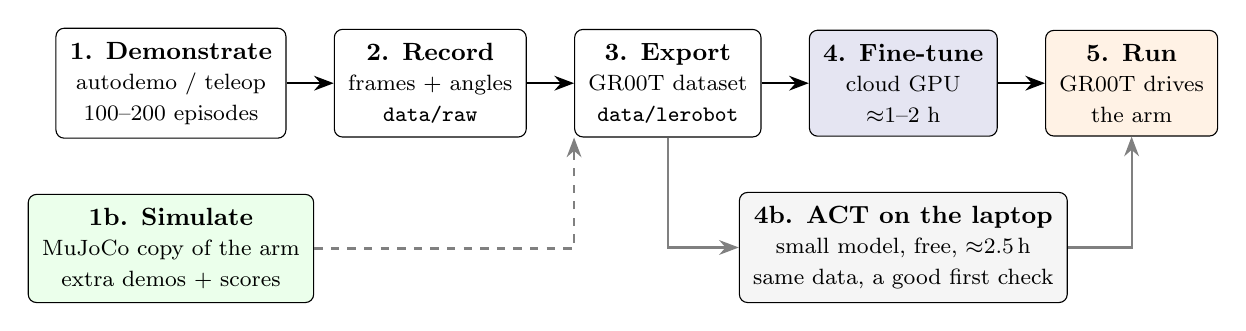
\begin{tikzpicture}[node distance=5mm and 6mm]
  \node[box] (a) {\textbf{1. Demonstrate}\\ \footnotesize autodemo / teleop\\ \footnotesize 100--200 episodes};
  \node[box,right=of a] (b) {\textbf{2. Record}\\ \footnotesize frames + angles\\ \footnotesize \file{data/raw}};
  \node[box,right=of b] (c) {\textbf{3. Export}\\ \footnotesize GR00T dataset\\ \footnotesize \file{data/lerobot}};
  \node[box,right=of c,fill=NavyBlue!10] (d) {\textbf{4. Fine-tune}\\ \footnotesize cloud GPU\\ \footnotesize $\approx$1--2 h};
  \node[box,right=of d,fill=orange!10] (e) {\textbf{5. Run}\\ \footnotesize GR00T drives\\ \footnotesize the arm};
  \foreach \x/\y in {a/b,b/c,c/d,d/e} \draw[arr] (\x) -- (\y);
  \node[box,below=7mm of d,fill=gray!8] (act) {\textbf{4b. ACT on the laptop}\\ \footnotesize small model, free, $\approx$2.5\,h\\ \footnotesize same data, a good first check};
  \draw[arr,gray] (c.south) |- (act.west);
  \draw[arr,gray] (act.east) -| (e.south);
  \node[box,below=7mm of a,fill=green!8] (sim) {\textbf{1b. Simulate}\\ \footnotesize MuJoCo copy of the arm\\ \footnotesize extra demos + scores};
  \draw[arr,gray,dashed] (sim.east) -| (c.south west);
\end{tikzpicture}
\caption{From demonstrations to a running policy. ACT \cite{act} is a much smaller imitation-learning model that trains on the laptop; it checks the data before paying for a GPU. The simulation (\cref{sec:sim}) adds demos and scores models once the real demos exist.}
\label{fig:pipeline}
\end{figure}

\section{Presenting it in a humanoids talk}
\label{sec:present}

\subsection{A 3-minute script}

\begin{say}
\begin{enumerate}[leftmargin=*]
\item \textbf{The problem.} ``A humanoid has to turn what it sees and what it's told into
  motor commands for dozens of joints. Writing that by hand doesn't scale. NVIDIA's answer is
  GR00T, a foundation model for robots.''
\item \textbf{Point at the arm.} ``This is a \$10 open-source arm, mobiobi's Easy Robot Arm: five hobby servos and a cheap webcam as
  the camera. GR00T doesn't care that it's small. The recipe is the same one used for humanoids.''
\item \textbf{Inputs and outputs} (\cref{fig:loop}). ``Three inputs: the camera image, an
  instruction in English, and the current joint angles. One output: a chunk of the next
  16 joint commands, about half a second of motion.''
\item \textbf{Two systems.} ``Inside, a vision-language model figures out \emph{what} to do,
  and a diffusion transformer turns that into \emph{how} the joints move. Slow thinking and
  fast moving.''
\item \textbf{New body.} ``GR00T has never seen this arm. I registered it as a new embodiment:
  4 joints, a gripper, one camera, and fine-tuned it on about 150 demonstrations, half picking
  the ball and half the block, each with its sentence. That took
  an hour or two on a rented GPU.''
\item \textbf{Demo} (\cref{sec:demo}).
\item \textbf{Back to humanoids.} ``A humanoid is the same loop with more joints, more cameras
  and much more data. Pretraining on many bodies is what lets each new body learn from only a
  handful of demonstrations.''
\end{enumerate}
\end{say}

\subsection{Live demo plan}
\label{sec:demo}
Pick the most ambitious option you have working, and keep the next one ready.
\begin{enumerate}
\item \textbf{GR00T live.} Start the cloud machine and \file{serve.sh} about 30 minutes before class, connect with
  \file{run_policy.py gr00t}. Needs internet. Put the ball and the block on two marked
  spots, ask the audience which one, and type it: \texttt{pick up the block}. When it's done it
  asks again, so swap the objects around and do the other one.
\item \textbf{ACT live (no internet).} Same pipeline, smaller model running on the laptop:
  \file{run_policy.py act}. Say clearly that this is the small model trained on the same data.
  ACT can't read words: it gets ``ball'' or ``block'' as a single number (0 or 1). That
  difference is a good point to make: GR00T understands the sentence, ACT only gets a switch.
\item \textbf{Scripted demo.} \file{autodemo.py --target block --spot C1 --other-spot A3}
  always works. Explain that this script is how the training demonstrations were collected,
  and that the learned policy never sees the spot names, only the camera image and the words.
\item \textbf{Video.} Screen-record a successful GR00T run the day before as a backup.
\end{enumerate}
Show the dataset too: open one recorded \file{episode_000000.mp4} to make ``demonstration
data'' concrete.

\subsection{Questions you might get}
\begin{description}[leftmargin=0pt,font=\normalfont\itshape]
\item[Why not just program the pick-up?] You can, and the scripted demo does. But that only
  works if the ball is exactly on a known spot. A learned policy reads the image, so the same
  approach scales to tasks nobody can script, like folding a shirt.
\item[How much data?] 100--200 demonstrations here, about half for each object. Pretraining
  is what makes that enough.
\item[Does it really understand the words?] Both objects are on the plate in every demo, so
  the only way to know which one to pick is the instruction. If it picks the right one after
  you swap their places, it's using the words and the image together.
\item[Why chunks of actions?] Smoother motion, fewer model calls, and the model commits to a
  plan. Re-planning every 8 steps still lets it correct mistakes.
\item[Does it generalise?] Within reason: other spots on the plate, small lighting changes.
  Not to a new task it was never shown.
\item[Did you train it in simulation?] The demos came from the real arm; a simulated copy
  (MuJoCo) added demos with the objects at more positions and scored each model automatically.
  The training is the same either way: copying demonstrations.
\item[Why the cloud?] Fine-tuning GR00T needs a GPU with about 40\,GB of memory and running it
  about 16\,GB; the laptop has 8\,GB. The cloud machine is only switched on while it's used.
\end{description}

%======================================================================
\part{Build and run instructions}
%======================================================================

\section{What you need}

\begin{table}[htbp]
\centering\small
\caption{Parts. Nothing exotic; most of it you already have. Beyond these, the only
possible cost is cloud GPU time for GR00T, which has free options (\cref{sec:cloud}).}
\begin{tabularx}{\linewidth}{@{}l c X@{}}
\toprule
Part & Qty & Notes \\
\midrule
SG90 micro servo, \textbf{180\textdegree} (with horns and screws) & 5 & base, shoulder, elbow, wrist, gripper.
  \textbf{Not} the 360\textdegree{} / ``continuous'' version, which looks the same but can't hold
  an angle (\cref{sec:servotest}). MG90S (same size, metal gears) also fits. The arm's design
  has room for a 6th (wrist roll); we leave it out \\
Arduino Nano + USB cable & 1 & the cable must carry data, not only charge \\
Adjustable bench power supply & 1 & set to 5.5\,V, current limit 3\,A \\
Breadboard + male--male jumper wires & -- & to share power between servos \\
Superglue (CA) & -- & optional: only if a part slips on its horn or the gripper turns \\
Orange soft foam ball (40\,mm) & 1 & squeezable PU/stress-ball foam: grips better and rolls less than a ping-pong ball. Keep it 40\,mm (the grip height and finger opening assume it); a ping-pong ball or two glued \file{12_ball_half} also work \\
Printed block (25\,mm cube) & 1 & \file{13_block}, in a colour that stands out from the ball
  and the plate (green, with an orange ball on a light grey plate). Avoid a white ball: it barely
  stands out from the light grey plate \\
USB webcam with monitor clip & 1 & ours: KitGody 1080p, 90\textdegree{} view. Plug and play.
  Its clip has a 1/4"-20 tripod hole underneath. A phone with a webcam app (Iriun, DroidCam,
  Phone Link) on \file{09_phone_cradle} also works \\
1/4"-20 screw, $\approx$3/8" (10\,mm) long & 1 & holds the webcam on \file{14_webcam_mount}. Hardware or camera store. A 1/2" screw works with a washer under its head \\
PLA filament & a few hundred g & Bambu printer; one 1\,kg spool is plenty \\
Optional: 470--1000\,$\mu$F capacitor & 1 & across the servo power rail; smooths current spikes \\
Optional: small elastic bands & -- & the author's tip: around the joints to damp vibration \\
\bottomrule
\end{tabularx}
\end{table}

\section{Printing}

The arm is mobiobi's \emph{Easy Robot Arm} \cite{easyarm}, printed without changes from the
author's files in \path{cad/stl_opensource/easy_robot_arm/}. The work cell (baseplate, camera
mast, phone cradle, cup) is ours, in \file{cad/stl}, generated from \file{cad/arm.py}.

\begin{table}[htbp]
\centering\small
\caption{Print list. Arm parts: the author's settings, PLA, 0.2\,mm layers, supports on,
10\% gyroid infill. Work-cell parts: PLA, 0.2\,mm, 3 walls, 20\% infill, no supports.}
\label{tab:print}
\begin{tabularx}{\linewidth}{@{}l c X@{}}
\toprule
File & Qty & What it is / how to print \\
\midrule
\multicolumn{3}{@{}l}{\emph{The arm} (\file{cad/stl_opensource/easy_robot_arm})} \\
\file{Base} & 1 & drum; the base servo sits inside \\
\file{BaseRotator} & 1 & turntable on the base servo; holds the shoulder servo \\
\file{BaseCap} & 1 & screw-on ring that holds the turntable on the drum \\
\file{Arm60mm} & 2 & upper arm and forearm (each carries the next servo) \\
\file{offAxis_gTrunkUndr} & 1 & wrist piece; hangs the gripper below the wrist axis \\
\file{gripperMount}, \file{gripperCap} & 1 each & hold the gripper servo; the cap clamps it to the wrist piece \\
\file{gripperOne}, \file{gripper_Two} & 1 each & geared fingers (they open sideways) \\
\file{gripperPinOne}, \file{gripperPinTwo} & 1 each & finger pivot pins \\
\midrule
\multicolumn{3}{@{}l}{\emph{The work cell} (\file{cad/stl})} \\
\file{07_baseplate} & 1 & flat; 250$\times$200\,mm, the longest print (15\% infill is fine) \\
\file{08_camera_mast} & 1 & standing up, 4 walls \\
\file{15_mast_extension} & 1 & goes between the mast's top and the webcam mount, lifting the camera 80\,mm; lying on one of its slanted faces, no supports. Print a second \file{10_pin} for it \\
\file{09_phone_cradle} & 1 & only if you use a phone as the camera; back face down \\
\file{14_webcam_mount} & 1 & the big flat face (with the square socket) on the bed; no supports \\
\file{10_pin} & 1 & lying flat \\
\file{11_cup} & 1 & upright, black \\
\file{12_ball_half} & 2 & only if you have no 40\,mm ball; open side down \\
\file{13_block} & 1 & the second object; contrasting colour, 15\% infill \\
\bottomrule
\end{tabularx}
\end{table}

\noindent Not needed: \file{BaseLeg} (the drum stands in a ring on the baseplate instead),
\file{Arm75mm}, \file{Arm90mm}, \file{gripperTrunk}, \file{offAxis_gTrunk},
\file{twistMount} and the two \file{28BYJ-48} stepper parts. The \file{00}--\file{06} files
in \file{cad/stl} are an older arm design and aren't used.

\begin{figure}[htbp]
\centering
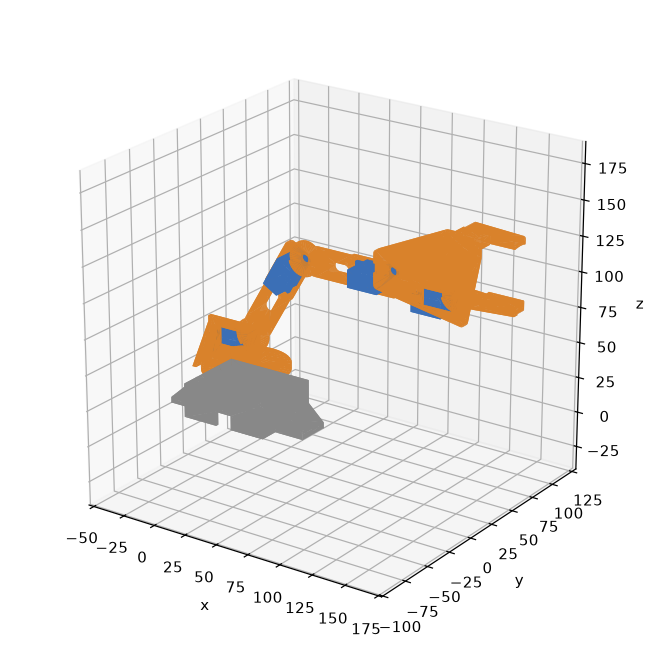
\includegraphics[width=0.47\linewidth,trim=60 60 60 60,clip]{arm_home}\hfill
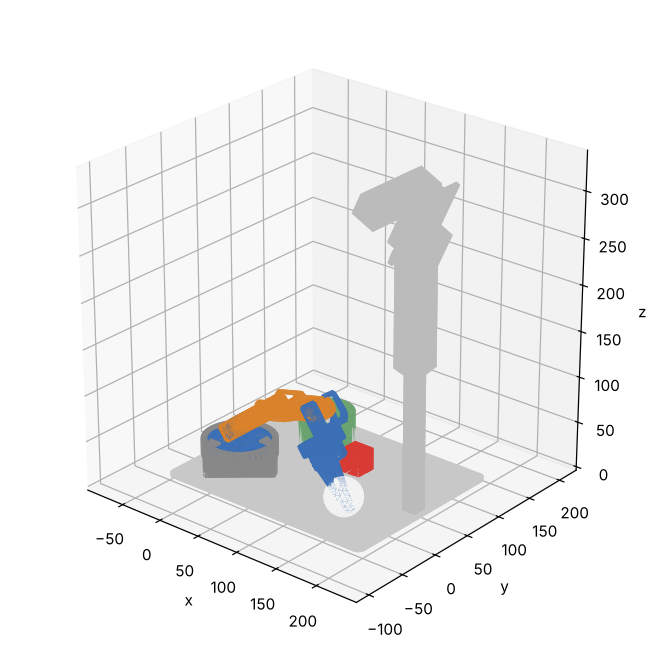
\includegraphics[width=0.47\linewidth,trim=60 60 60 60,clip]{work_cell}
\caption{Left: the Easy Robot Arm in its home pose, built from the author's 3D model with two
60\,mm links. Right: the work cell with the baseplate, cup and the webcam on its mast (with the
80\,mm extension on top), the arm
gripping the ball on C1 with the block on A3. \file{cad/assembly.py} checks the arm against
itself and the work cell: every marked spot (ball and block), the lift above it and the drop
over the cup are clear, and the gripper never touches the other object in any layout the demos
use.}
\label{fig:cell}
\end{figure}

\section{Laptop software setup}

\begin{enumerate}
\item Install \textbf{uv} (Python manager) and \textbf{Arduino CLI} in PowerShell:
\begin{cmd}
powershell -c "irm https://astral.sh/uv/install.ps1 | iex"
winget install ArduinoSA.CLI
\end{cmd}
\item Get the code and install the Python packages:
\begin{cmd}
gh repo clone Yishane/gr00t-arm
cd gr00t-arm\software
uv sync
\end{cmd}
\item Plug in the USB webcam; it needs no driver. The laptop's own camera is usually index 0
  and the webcam 1 (\texttt{--camera 1}). Using a phone instead: install \textbf{Iriun Webcam}
  or \textbf{DroidCam} on the phone and the PC (or Windows Phone Link on Android); it shows up
  as a normal webcam too.
\end{enumerate}

\section{Wiring}

\begin{figure}[htbp]
\centering
\resizebox{\linewidth}{!}{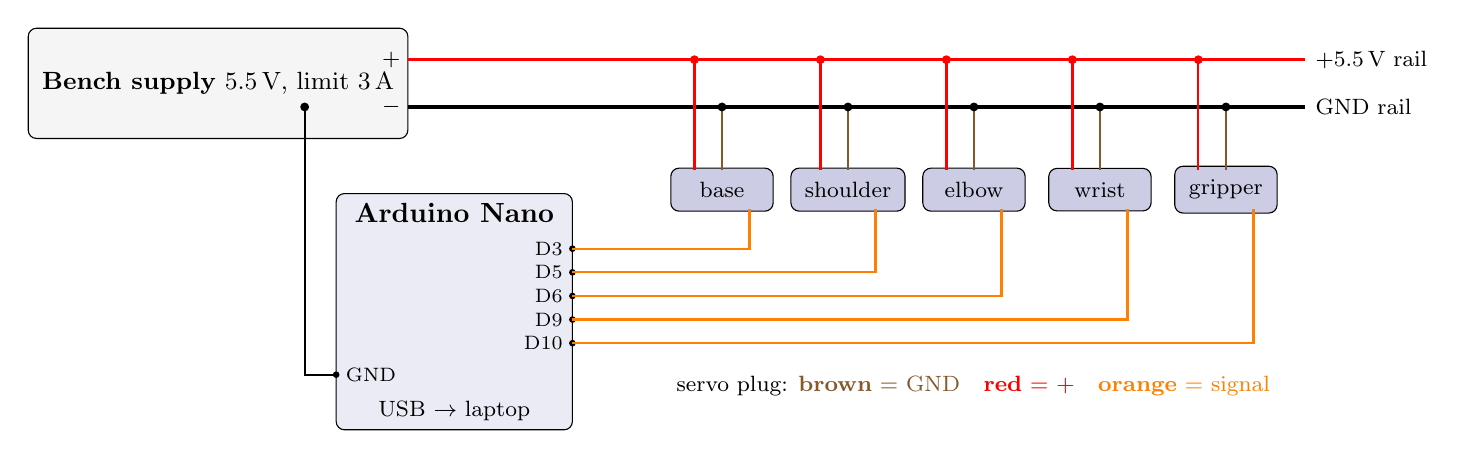
\begin{tikzpicture}[font=\small,x=1cm,y=1cm]
  \def\yp{3.0}\def\yg{2.4}
  % bench supply
  \node[box,fill=gray!8,minimum width=24mm,minimum height=14mm] (psu) at (0.6,2.7)
    {\textbf{Bench supply}\ 5.5\,V, limit 3\,A};
  % rails
  \draw[red,very thick] (psu.east |- 0,\yp) node[left=-1pt,black,font=\footnotesize]{$+$} -- (14.4,\yp)
     node[right,black,font=\footnotesize]{$+$5.5\,V rail};
  \draw[very thick] (psu.east |- 0,\yg) node[left=-1pt,font=\footnotesize]{$-$} -- (14.4,\yg)
     node[right,font=\footnotesize]{GND rail};
  % nano
  \node[box,fill=NavyBlue!8,minimum width=30mm,minimum height=30mm] (nano) at (3.6,-0.2) {};
  \node[font=\bfseries,anchor=north] at (nano.north) {Arduino Nano};
  \node[font=\footnotesize,anchor=south] at (nano.south) {USB $\rightarrow$ laptop};
  \foreach \i/\p in {0/D3,1/D5,2/D6,3/D9,4/D10}{
    \pgfmathsetmacro{\py}{0.6-0.3*\i}
    \node[font=\scriptsize,anchor=east] at (5.1,\py) {\p};
    \fill (5.1,\py) circle (1.2pt);
  }
  \node[font=\scriptsize,anchor=west] at (2.1,-1.0) {GND};
  \fill (2.1,-1.0) circle (1.2pt);
  \draw[thick] (2.1,-1.0) -- (1.7,-1.0) -- (1.7,\yg);
  \fill (1.7,\yg) circle (1.6pt);
  % servos
  \foreach \i/\n in {0/base,1/shoulder,2/elbow,3/wrist,4/gripper}{
    \pgfmathsetmacro{\sx}{7.0+1.6*\i}
    \pgfmathsetmacro{\py}{0.6-0.3*\i}
    \node[box,fill=NavyBlue!20,minimum width=13mm,font=\footnotesize] (s\i) at (\sx,1.35) {\n};
    \draw[red,thick] (\sx-0.35,1.6) -- (\sx-0.35,\yp);  \fill[red] (\sx-0.35,\yp) circle (1.6pt);
    \draw[brown!70!black,thick] (\sx,1.6) -- (\sx,\yg);  \fill (\sx,\yg) circle (1.6pt);
    \draw[orange,thick] (\sx+0.35,1.1) -- (\sx+0.35,\py) -- (5.1,\py);
  }
  \node[font=\footnotesize,anchor=north west,align=left] at (6.3,-0.9)
    {servo plug: \textcolor{brown!70!black}{\textbf{brown} = GND}\quad
     \textcolor{red}{\textbf{red} = +}\quad \textcolor{orange}{\textbf{orange} = signal}};
\end{tikzpicture}}
\caption{Wiring. Servo power comes from the bench supply, \emph{never} from the Nano's 5V
pin. The Nano's GND must connect to the supply's negative so the signals have a common
reference. Orange signal wires go to D3, D5, D6, D9, D10 in the order base, shoulder, elbow,
wrist, gripper.}
\label{fig:wiring}
\end{figure}

\begin{enumerate}
\item Set the bench supply to \textbf{5.5\,V} with the current limit at \textbf{3\,A}, output off.
\item Bench supply $+$ to the breadboard's red rail, $-$ to the blue rail. (Optional: the
  capacitor across the two rails, its stripe/negative leg to the blue rail.)
\item Each servo: red to the red rail, brown to the blue rail (use jumpers into the servo's
  3-pin plug), orange to its Nano pin from \cref{fig:wiring}.
\item One jumper from a Nano GND pin to the blue rail.
\item Nano to the laptop by USB.
\end{enumerate}
\begin{note}[Why the separate supply]
Five SG90s can pull over 2\,A when they start moving together. USB gives 0.5\,A: the Nano
would reset and the arm would twitch. If the supply hits its current limit (the CC light
comes on) something is jammed; turn it off and check.
\end{note}

\subsection{Upload the firmware}
Find the Nano's port in Device Manager $\rightarrow$ Ports (e.g.\ COM3), then:
\begin{cmd}
cd gr00t-arm\firmware
.\upload.ps1 COM3
\end{cmd}
The script tries the ``old bootloader'' (most Nano clones) and then the new one.
\textbf{Or with the Arduino IDE:} open \file{firmware/arm/arm.ino}, pick Tools $\rightarrow$ Board
$\rightarrow$ Arduino Nano, Processor $\rightarrow$ ATmega328P (Old Bootloader) (if the upload fails,
plain ATmega328P), Port $\rightarrow$ your COM port, then Upload. The firmware
listens on USB serial for lines like \texttt{90,90,90,90,125} (five angles) and moves each
servo smoothly toward its target.

\subsection{Check every servo before you fit it}
\label{sec:servotest}
SG90s also come in a 360\textdegree{} ``continuous'' version that looks identical. It can't
hold an angle: it treats 90 as ``stop'' and anything else as ``keep spinning''. Test each servo
on its own, before it goes into the arm and with no horn on: send it 0, then 180 (in
\file{calibrate.py}: \texttt{s 0 0}, then \texttt{s 0 180} with the servo on D3). A good servo
turns to one end and \emph{stops}, then to the other end and stops. If it keeps spinning, put it
aside. Label each good servo with its joint as you plug it in.

\section{How the laptop talks to the Nano}
\label{sec:serial}

The laptop does all the thinking; the Nano only moves servos. About 30 times a second
the laptop sends the Nano one line of text over USB with five angles in it, and the Nano
moves the five servos toward them. GR00T never talks to the Nano: it runs on the cloud GPU,
answers the laptop, and the laptop passes the answer on. With ACT the model runs on the
laptop instead and everything below stays the same.

\begin{figure}[htbp]
\centering
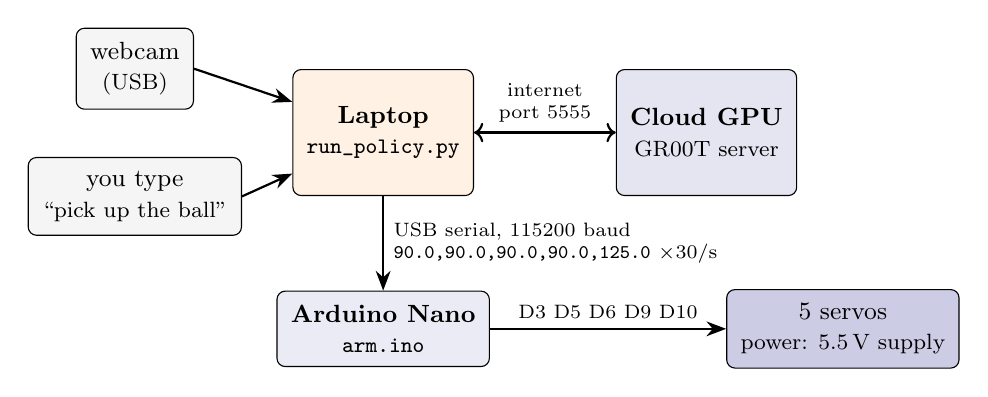
\begin{tikzpicture}[node distance=6mm and 10mm]
  \node[box,fill=gray!8] (cam) {webcam\\ \footnotesize (USB)};
  \node[box,below=of cam,fill=gray!8] (you) {you type\\ \footnotesize ``pick up the ball''};
  \node[box,right=20mm of $(cam)!0.5!(you)$,fill=orange!10,minimum height=16mm] (lap)
    {\textbf{Laptop}\\ \footnotesize \file{run_policy.py}};
  \node[box,right=18mm of lap,fill=NavyBlue!10,minimum height=16mm] (gpu)
    {\textbf{Cloud GPU}\\ \footnotesize GR00T server};
  \node[box,below=12mm of lap,fill=NavyBlue!8] (nano) {\textbf{Arduino Nano}\\ \footnotesize \file{arm.ino}};
  \node[box,right=30mm of nano,fill=NavyBlue!20] (srv) {5 servos\\ \footnotesize power: 5.5\,V supply};
  \draw[arr] (cam.east) -- (lap);
  \draw[arr] (you.east) -- (lap);
  \draw[arr,<->] (lap) -- node[above,font=\scriptsize,align=center]{internet\\port 5555} (gpu);
  \draw[arr] (lap) -- node[right,font=\scriptsize,align=left]{USB serial, 115200 baud\\
    \texttt{90.0,90.0,90.0,90.0,125.0} $\times$30/s} (nano);
  \draw[arr] (nano) -- node[above,font=\scriptsize]{D3 D5 D6 D9 D10} (srv);
\end{tikzpicture}
\caption{Who talks to whom. The Nano only ever sees five angles per line.}
\label{fig:serial}
\end{figure}

\subsection{The USB cable is a serial port}
\begin{itemize}
\item Plugged in, the Nano shows up as a COM port. The Python scripts find it by name
  (``Arduino'', ``CH340'' or ``USB''); pass \texttt{--port COM5} if they pick the wrong one.
\item Speed is \textbf{115200 baud} on both sides (\texttt{BAUD} in \file{config.py},
  \texttt{Serial.begin} in \file{arm.ino}).
\item Opening a port normally \textbf{resets the Nano} (servos twitch, then snap to 90\textdegree).
  The Python scripts open it with the reset line (DTR) held off so it keeps running, ask
  \texttt{?} until it answers, and set the speed back to 180\textdegree/s. When the Nano does start
  (power-up, reset button, Arduino Serial Monitor) it prints \texttt{READY} and moves every servo to 90\textdegree.
\item Only one program can hold the port. Close the Arduino Serial Monitor before running Python.
\end{itemize}

\subsection{The messages}
Plain text, one command per line:

\begin{center}\small
\begin{tabularx}{\linewidth}{@{}p{4.6cm}X@{}}
\toprule
Laptop sends & The Nano \\
\midrule
\texttt{90,120.5,45,90,125} & sets new target angles (degrees) for base, shoulder, elbow, wrist, gripper \\
\texttt{S 120} & sets the top servo speed to 120\textdegree/s (default 180) \\
\texttt{?} & replies \texttt{P a0,a1,a2,a3,a4}, the angles it is at now (for debugging; Python doesn't use it) \\
\bottomrule
\end{tabularx}
\end{center}
A line without exactly five numbers is ignored. You can type these into the Arduino Serial
Monitor (115200 baud, ``Newline'' ending) to test the arm with no Python at all.

\subsection{What the Nano does with them}
\begin{enumerate}
\item Reads characters up to a newline, splits the line on commas.
\item Clamps each angle to 0--180\textdegree{} and stores it as that servo's \emph{target}.
\item Every 10\,ms moves each servo a small step toward its target, at most 180\textdegree/s, so a
  big jump in the commands becomes a smooth swing instead of a slam.
\item Turns each angle into a pulse (0\textdegree{} = 500\,\textmu s, 180\textdegree{} = 2400\,\textmu s)
  on that servo's signal pin.
\end{enumerate}
The Nano knows nothing about kinematics, the camera or GR00T. It also can't tell where the
servos really are: SG90s don't report their position, so it only remembers what it sent.

\subsection{Where the numbers come from}
The numbers on the wire are always \emph{servo} angles (0--180\textdegree), not joint angles.
\begin{itemize}
\item \file{teleop.py} and \file{autodemo.py} think in gripper positions ($x,y,z$).
  \file{kinematics.py} turns a position into joint angles, then into servo angles using
  \file{calibration.json} (each servo's direction and zero).
\item \file{run_policy.py}: the model was trained on servo angles, so its answer already
  \emph{is} servo angles. The laptop clips each to 0--180\textdegree{} and sends it on.
\end{itemize}

\subsection{The loop when GR00T drives}
\begin{enumerate}
\item Grab a 640$\times$480 photo from the webcam.
\item Package the photo, the five angles last sent, and your sentence.
\item Send it to the GR00T server (\file{policy_client.py}: a ZeroMQ request on port 5555
  through the SSH tunnel). GR00T replies with \textbf{16} future steps of five angles each.
\item Send the first \textbf{8} steps to the Nano, one line every $1/30$\,s (about 0.27\,s).
\item Repeat with a new photo, for 20\,s (\texttt{--seconds}) or until Ctrl+C, then go home.
\end{enumerate}
Steps 1--3 for the next chunk run \emph{while} step 4 is still playing: once what is left to
play takes about as long as the last call did ($\sim$0.28\,s to the cloud), the next request
goes out in the background. The new chunk skips the steps planned for the time the call was
out, so the arm doesn't stop between chunks; \texttt{--no-pipeline} turns this off.
The ``state'' GR00T sees is the angles last \emph{sent}, not measured ones, since the servos
can't report back. The recordings were made the same way (every $1/30$\,s \file{recorder.py}
saves the photo and the five angles just sent), so the model gets the same kind of state it
learned from.

\begin{note}[Power is a separate path]
The USB cable only powers the Nano's chip and carries data. The servos run from the bench
supply, and the supply's ground must be wired to the Nano's GND (\cref{fig:wiring}). Without
the common ground the signal pulses have no shared reference and the servos jitter or don't move.
\end{note}

\section{Assembly}

The author gives no written steps. The parts are made to need only what comes with the SG90s
(the horns and screws), and every servo slides into a pocket so it can be swapped. Look at
the photos on the Printables page \cite{easyarm} for how each piece sits.

\begin{note}[The one rule]
Every servo must be at \textbf{90\,\textdegree} when the part it drives goes on, with that
part in the \textbf{home pose}: arm facing forward, upper arm straight up, forearm level and
pointing forward, gripper level and in line with the forearm, fingers closed. The software
assumes this; get it right and calibration is only small trims.
\end{note}

\begin{enumerate}
\item \textbf{Center all servos.} Wire all five servos with nothing attached, power on, and run
\begin{cmd}
cd gr00t-arm\software
uv run calibrate.py
> center
\end{cmd}
All five turn to 90\,\textdegree. Leave them powered while fitting parts, and don't turn a
shaft by hand.
\item \textbf{Base.} Base servo into the drum (\file{Base}), shaft up. Put the turntable
  (\file{BaseRotator}) on its horn so the arm will swing forward and back. Screw
  \file{BaseCap} over it onto the drum. Leave the \file{BaseLeg} feet off.
\item \textbf{Shoulder.} Shoulder servo into the turntable. The first \file{Arm60mm} (upper
  arm) onto its horn, pointing \emph{straight up}.
\item \textbf{Elbow.} Elbow servo into the top of the upper arm. The second \file{Arm60mm}
  (forearm) onto its horn, pointing \emph{forward, level}.
\item \textbf{Wrist.} Wrist servo into the end of the forearm. The wrist piece
  (\file{offAxis_gTrunkUndr}) onto its horn so the gripper will hang \emph{below} the
  forearm, pointing forward and level.
\item \textbf{Gripper.} Gripper servo into \file{gripperMount}; the fingers on their pins with
  the gears meshed and the fingers \emph{closed}; then clamp \file{gripperMount} to the wrist
  piece with \file{gripperCap}.
\item \textbf{No wrist-roll servo.} The design has room for one between the wrist piece and
  the gripper; we leave it out so the software stays at 5 joints. If the gripper turns on the
  wrist piece, put a drop of superglue between the two discs.
\item \textbf{Work cell.} Stand the drum in the ring on the baseplate (spots A1--C3 in front,
  the cup ring to the left) and fix it with double-sided tape or a few dots of hot glue, so
  the base servo turns the arm and not the drum. Push the mast into its socket, a pin into the mast top, the extension
  (\file{15_mast_extension}) onto that pin, a second pin into the extension's top, and
  \file{14_webcam_mount} onto that pin, its plate on the far side from the arm (or, with a phone, the
  phone cradle onto the pin). Clamp or tape the baseplate's back edge to
  the desk.
\item \textbf{Camera.} Fold the webcam's clip shut (the back leg flat under the top bar), rest
  the folded clip on the mount's plate against the lip, lens facing the arm, and screw it on through
  the slot from behind. A zip tie through the side slots is an extra hold. Set the head's own hinge
  straight, then do \cref{sec:camsetup}. (Phone: landscape on the cradle, resting on the lip, rear camera near the
  lip.)
\item \textbf{Cables.} Leave slack at every joint so nothing pulls when the arm turns.
\end{enumerate}

\subsection{Camera setup and framing check}
\label{sec:camsetup}
\begin{enumerate}
\item \textbf{Webcam:} plug it in; nothing to set up. \file{14_webcam_mount} on the mast and
  its extension holds it about 325\,mm above the plate, looking 65\textdegree{} down. On the 3D
  model that keeps the fingers, all nine spots and the cup in view during every scripted pick,
  and the elbow and wrist too (from 80\,mm lower, without the extension, they left the top of the
  picture in a quarter to a third of the frames). The plate sits in the lower half of the picture: tilt the
  head about 5--10\textdegree{} further down on its own $\pm$20\textdegree{} hinge to centre it.
  Once the check below passes, put a strip of tape across the hinge so it can't move.
  \textbf{Phone:} in the webcam app pick the \textbf{rear} camera and, if it lets you choose,
  the \textbf{0.5$\times$ (ultra-wide)} lens. 1$\times$ was tight from the phone cradle before the extension (the
  fingers would leave the top of the picture in roughly a quarter of the frames).
  Any resolution of 640$\times$480 or more is fine; the code scales it to 640$\times$480.
\item Find the camera index and see the live picture:
\begin{cmd}
uv run teleop.py --camera 1
\end{cmd}
  The window shows what the camera sees. Wrong camera or ``didn't open''? Try \texttt{--camera 0} or \texttt{2}.
\item \textbf{Framing check.} Press \key{H} (home), then drive the gripper with
  \key{W}\key{A}\key{S}\key{D} and \key{F} down to the corner spots A1 and C3 and over the cup,
  and with \key{R} up to about $z = 95$ (shown at the bottom of the window). The \emph{fingers},
  all nine spots and the cup must stay in the picture. The elbow and upper arm going off the
  top is fine: the model gets those joints as angles anyway.
\item If the fingers leave the picture: tilt the webcam's head on its hinge (or use 0.5$\times$ on a phone), or
  tell Claude what is cut off so the mount can be changed and reprinted.
\item Once it looks right, don't touch it: same camera, same position, same lighting for
  every recording and for the live demo. If the app has focus or exposure lock, turn it on.
\end{enumerate}

\begin{note}[If the shoulder struggles]
The author notes the shoulder servo works hardest. If it sags or buzzes, swap just that one
for an MG90S (same size, metal gears, no code changes). Small elastic bands around the
joints, as in the author's photos, damp vibration.
\end{note}

\section{Calibration}

Still in \file{calibrate.py}:
\begin{enumerate}
\item \texttt{home} --- the arm should go to the home pose.
\item \texttt{test} --- moves each joint a little and tells you which way it should go. If one
  goes the wrong way, type \texttt{flip <joint>} (0 base, 1 shoulder, 2 elbow, 3 wrist).
\item If a joint is a few degrees off in the home pose: \texttt{trim <joint> <degrees>}, e.g.\
  \texttt{trim 1 -4}.
\item Gripper: \texttt{s 4 <deg>} to try angles. Find an angle that is well open, and one that
  squeezes the \emph{block} firmly (it's the smaller object, so this also grips the ball);
  set them with \texttt{grip open 125} and \texttt{grip closed 85} (your numbers). The
  fingers open sideways; check with the block and then the ball held between them. If the
  servo buzzes hard on the ball, tell Claude: the ball can get its own closed angle.
\item \texttt{save}, then \texttt{quit}. This writes \file{software/calibration.json}.
\end{enumerate}
\begin{note}[Check the tool point]
The arm's lengths in \file{software/config.py} were measured from the author's 3D model, not
from your printed arm. In \cref{sec:first}, if the fingers close a little in front of, behind,
above or below the ball, tell Claude how far off it is; \texttt{L\_TOOL} (along the gripper)
and \texttt{TOOL\_UP} (how far the fingers hang below the wrist) get a small trim.
\end{note}

\section{First moves}
\label{sec:first}

\begin{cmd}
uv run autodemo.py --spot B2 --camera 1
\end{cmd}
Put the ball on spot B2 first. The arm should pick it up and drop it in the cup. Then the
block, with the ball on another spot:
\begin{cmd}
uv run autodemo.py --target block --spot C1 --other-spot A3 --camera 1
\end{cmd}
Turn the block so one face points at the arm's base: the fingers close sideways. Then try
driving it yourself:
\begin{cmd}
uv run teleop.py --camera 1
\end{cmd}
Click the window, then: \key{W}/\key{S} forward/back, \key{A}/\key{D} left/right,
\key{R}/\key{F} up/down, \key{Q}/\key{E} tilt the gripper, \key{Space} open/close,
\key{H} home, \key{Esc} quit. If it says ``can't reach that'', the target is outside the arm's
reach or would hit the plate; it refuses rather than crashing. Add \texttt{--sim} to any script
to try it without hardware.

\section{Collecting demonstrations}

\begin{enumerate}
\item \textbf{Automatic (recommended):}
\begin{cmd}
uv run autodemo.py --record 150 --camera 1
\end{cmd}
  Each time it tells you where to put the ball and the block and which one it will pick, e.g.\
  \texttt{block on C1, ball on A3 -> "pick up the block"}. Place both, press Enter, and it
  picks and places while recording, saving the instruction with the demo. It picks the ball or
  the block about half the time each. After each pick it asks \texttt{keep it? [Y/n]}: press
  Enter to keep the demo, or type \texttt{n} if it missed the grip, dropped the object or
  knocked the other one, and that demo is thrown away. \texttt{--record 150} keeps going until
  150 demos are kept. Aim for 100--200 (about 20 seconds each, so 150 take under an hour;
  split it into sessions, it keeps numbering where it left off).
\item \textbf{By hand (optional, adds variety):} in \file{teleop.py}, \key{T} switches the
  instruction between ``pick up the ball'' and ``pick up the block'' (shown at the top of the
  window), \key{Enter} starts a recording, \key{Enter} again saves it, \key{Backspace} throws
  it away. Always pick the object the instruction names.
\end{enumerate}
\begin{note}[Good data]
Keep the camera, lighting and cup exactly where they will be during the demo. Both objects
are on the plate in every demo; the middle spot B2 isn't used because it's too close to the
others. Place the objects a little off-center sometimes, with a block face towards the base.
Answer \texttt{n} to every demo that went wrong: the model copies whatever it is shown,
mistakes included. (A bad demo you only notice later: delete its folder from
\file{data/raw/pick_ball}.)
\end{note}
Then export for GR00T:
\begin{cmd}
uv run export_dataset.py
\end{cmd}
This writes \file{data/lerobot/pick_ball} (\cref{tab:map}). GR00T's own data loader was used
to check this format.

\section{Training ACT on the laptop (free, optional but recommended)}

\begin{cmd}
cd software\act
uv sync
uv run export_act.py
uv run train_act.py --steps 20000
uv run ..\run_policy.py act --camera 1 ^
    --checkpoint ..\..\outputs\act\pick_ball\checkpoints\020000\pretrained_model
\end{cmd}
Training runs at about 2.3 steps per second on the RTX 5050 (about 2.5 hours for 20k steps).
It asks for an instruction; type \texttt{pick up the ball} or \texttt{pick up the block} (or just
\texttt{ball} / \texttt{block}). Each runs for 20 seconds (\texttt{--seconds}), then the arm goes
home and it asks again; \texttt{q} quits. If ACT picks up the right object, the data is good
and GR00T will learn from it too.

\subsection{Learning from its own runs}
\label{sec:selfrecord}
The trained policy can record its own runs, and the good ones become extra training data:
\begin{cmd}
uv run ..\run_policy.py act --camera 1 --record pick_ball ^
    --checkpoint ..\..\outputs\act\pick_ball\checkpoints\020000\pretrained_model
\end{cmd}
\begin{enumerate}
\item Type an instruction as usual. Every step the arm plays is saved: the camera frame, the
  five angles last sent (the state) and the five angles sent now (the action), exactly like a
  demo, tagged \texttt{"source": "policy"} in its \file{meta.json}. If the safety check
  cut a step short, the safe move the arm actually made is what gets saved.
\item Press Ctrl+C as soon as the object is in the cup, so the seconds after it aren't saved.
  The arm goes home and asks \texttt{keep it? [Y/n]}.
\item Keep a run \emph{only} if it picked the right object cleanly. Training on its successes
  makes it better (it sees more object positions it handled well); training on its failures
  would teach it its own mistakes. Keep ball and block runs roughly even.
\end{enumerate}
\texttt{--record pick\_ball} puts the runs next to your demos, numbered after them, so the
next export uses both; \texttt{--record} alone saves them to a separate
\file{pick_ball_policy} set to look at first. Collect a batch (30--50 kept runs in one
sitting), then export and train once, overnight. \file{train_act.py} won't overwrite an
earlier model, so rename the old one first (and keep it to compare):
\begin{cmd}
ren ..\..\outputs\act\pick_ball pick_ball_round1
uv run export_act.py
uv run train_act.py --steps 20000
\end{cmd}
The same works with GR00T: add \texttt{--record pick\_ball} to \texttt{run\_policy.py gr00t},
then export with \file{export_dataset.py} and fine-tune again. This only adds runs where the policy
\emph{already} succeeds, so it fills in positions near what it can do; for positions it fails
at, it needs new demos (or the simulator, \cref{sec:sim}).

\section{Fine-tuning and running GR00T in the cloud}
\label{sec:cloud}

\subsection{One-time accounts (you do these)}
\begin{enumerate}
\item \textbf{Hugging Face}: make a free account at \url{https://huggingface.co}, open
  \url{https://huggingface.co/nvidia/Cosmos-Reason2-2B} and request access (GR00T is built on
  it). Then create an access token (Settings $\rightarrow$ Access Tokens, ``read'').
\item \textbf{GPU time.} Fine-tuning needs a GPU with at least 40\,GB (L40S, A100 or H100).
  Try free credits first. \textbf{Lightning AI}'s free plan gives monthly credits and a
  Studio you can SSH into, so the steps below work unchanged. \textbf{Modal}'s free plan gives
  about \$30 a month, but it needs a small wrapper script first. Otherwise, rent a machine
  on a paid cloud such as RunPod or Lambda. Free 16\,GB GPUs (Colab, Kaggle) are too small.
\end{enumerate}

\begin{note}[This is the only step that can cost money]
Everything before this section is free. If you don't want to pay and there are no free
credits, stop after ACT: it uses the same data and the same control loop, and it is a
fine live demo (\cref{sec:demo}, option 2). Check the free plans' current terms on their
pricing pages before signing up.
\end{note}

\subsection{Steps}
\textbf{Do a dry run first:} \file{docs/gr00t_dry_run.md} runs these same steps on a small fake
dataset (\file{software/gr00t/dryrun}) in about an hour, so setup problems show up before the real data does.
\begin{enumerate}
\item Start a Linux GPU machine (Ubuntu, L40S/A100/H100, $\ge$100\,GB disk). Note its SSH
  address and port.
\item Copy the GR00T scripts and the dataset up (from the \file{gr00t-arm} folder):
\begin{cmd}
scp -P <port> -r software\gr00t data\lerobot\pick_ball root@<ip>:~/
\end{cmd}
\item Log in and set up (installs GR00T and downloads the base model, $\approx$20 min):
\begin{cmd}
ssh -p <port> root@<ip>
export HF_TOKEN=hf_your_token
bash ~/gr00t/setup_cloud.sh
\end{cmd}
\item Fine-tune (about 1--2 hours; use \texttt{tmux} so it survives a disconnect):
\begin{cmd}
tmux
bash ~/gr00t/finetune.sh ~/pick_ball
\end{cmd}
  At the end it plots predicted vs.\ recorded actions for episode 0 in \file{/tmp/open_loop_eval}.
  The lines should overlap. Flat predicted lines mean something is wrong with the data.
\item Serve the model:
\begin{cmd}
bash ~/gr00t/serve.sh
\end{cmd}
\item On the laptop, open a tunnel in one terminal and run the arm in another:
\begin{cmd}
ssh -p <port> -L 5555:localhost:5555 root@<ip>
uv run run_policy.py gr00t --host localhost --camera 1
\end{cmd}
  Type the instruction at the \texttt{instruction>} prompt, the same as for ACT.
\item \textbf{Stop the cloud machine when you're done}: it bills by the hour. You don't keep it
  running until the presentation: turn it on only to fine-tune, to test, and on demo day.
  Running the trained model needs far less GPU memory than training it, so a smaller, cheaper
  GPU (around 16\,GB) is usually enough then. The laptop's RTX 5050 has 8\,GB, which is probably
  too little, but it's worth one try once the model is trained.
\end{enumerate}

\begin{note}[Cost and time]
A paid cloud GPU costs roughly \$1--3 per hour. Setup plus one fine-tune plus testing is a
few hours, so budget \$10--20 for the first run, or use free credits if they cover it. Download the checkpoint folder
(\file{~/gr00t_arm_ckpt}) if you want to reuse it later without retraining.
\end{note}

\section{Simulation (MuJoCo): more demos and automatic testing}
\label{sec:sim}

Once the real demos are recorded and ACT (and GR00T) have been trained on them, a simulated
copy of the arm can add two things the real arm can't do quickly: hundreds of extra demos with
the objects \emph{anywhere} on the plate, and an automatic score for every trained model. It
runs on the laptop, costs nothing, and the real arm can stay switched off.

\begin{note}[What ``training in simulation'' means here]
Training itself doesn't happen \emph{inside} the simulator: ACT and GR00T still learn by copying
recorded demos, on the laptop GPU or the cloud GPU, exactly as before. The simulator
\emph{makes} demos (the same kind of recording as on the real arm) and \emph{tests} models
(it knows where the ball ended up). This is also how GR00T itself was built: its pretraining mixes
real robot data with simulated robots. Your real demos stay in the mix: the simulator never
looks or behaves exactly like the real arm, and the real demos are what teach the model the
real thing.
\end{note}

\begin{figure}[htbp]
\centering
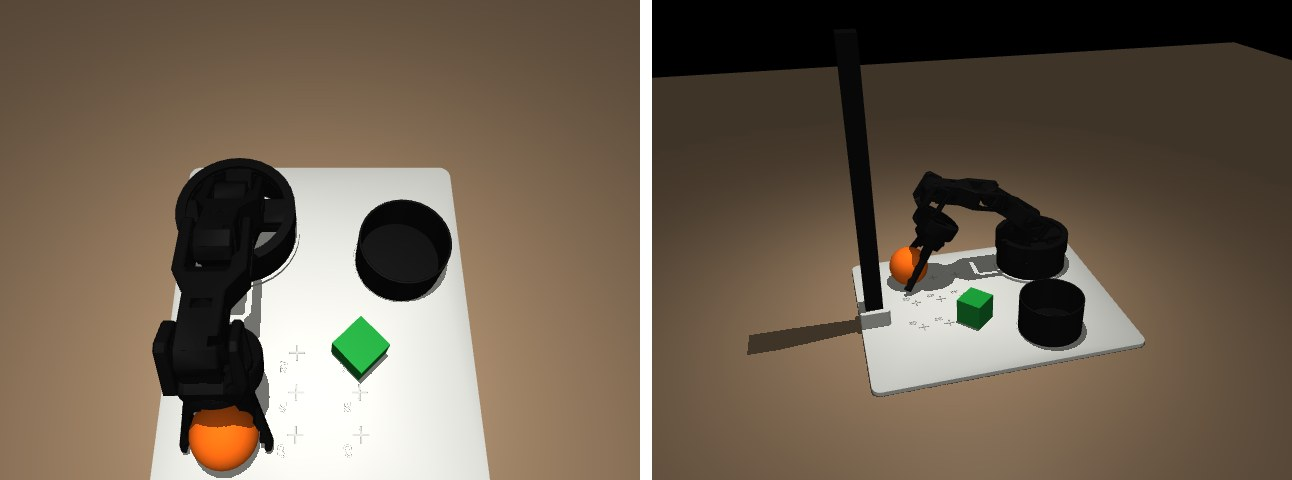
\includegraphics[width=\linewidth]{sim_views}
\caption{The simulation, rendered by \file{software/sim.py}. Left: what the simulated webcam
sees as the arm reaches for the ball on C1 (this is the image the model gets). Right: the same
moment from another angle. The arm's parts are the author's 3D model; the plate, cup, ball and
block are ours.}
\label{fig:sim}
\end{figure}

\subsection{How the simulation works}
\begin{description}[leftmargin=0pt]
\item[MuJoCo.] A free physics engine (\texttt{pip install mujoco}, installed by \texttt{uv sync}).
  \file{sim.py} describes the work cell to it: the arm's moving parts, the plate, the cup, the
  ball and the block. MuJoCo works out how they move and collide 500 times a simulated second
  and draws what a camera would see.
\item[The arm.] Each part is the author's 3D model, on joints placed with the numbers in
  \file{config.py}: shoulder 54\,mm above the plate, two 60\,mm links, tool point 86.5\,mm
  along the gripper and 24.75\,mm below the wrist. So the simulated gripper is where
  \file{kinematics.py} says it is. (The parts were converted once, by
  \file{cad/sim_meshes.py}, into the files in \file{software/sim_assets}.)
\item[Same commands as the real arm.] Scripts send the simulated arm the same five servo angles
  they send the Nano. \file{sim.py} turns them into joint angles with \emph{your}
  \file{calibration.json} (each servo's direction and zero), the same way \file{kinematics.py}
  does. So a recording made in the simulator has the same numbers as one made on the real arm,
  and the two can be trained on together. (Run the simulator on the laptop that has the
  calibration file.)
\item[The servos.] Like the firmware, each servo's target moves at most 180\textdegree/s, in
  10\,ms steps (\cref{sec:serial}). A simulated SG90 then follows it with limited strength
  (0.18\,N\,m, an SG90's stall torque), so the arm sags a few millimetres under its own weight,
  as the real one does (about 4\,mm at the tool in the home pose).
\item[The gripper.] The two geared fingers turn on their pins, mirrored, as the gears make
  them. Your calibrated ``open'' angle opens each finger 30\textdegree; your ``closed'' angle
  aims for 6\textdegree, a little narrower than the block, so the fingers stop on the object
  and squeeze it with the servo's limited force (on the block at about 12\textdegree, on the
  ball at 13--16\textdegree), like the real calibration.
\item[The objects.] A 40\,mm ball and a 25\,mm block (6\,g each), with grip and some rolling
  resistance like the foam ball. The block is turned with a face toward the base, as you place
  it. The arm collides with the plate, the cup, the mast and the objects, and the gripper with the
  base drum; the arm's parts don't collide with each other (the joint limits already stop that on
  the real arm).
\item[The camera.] A 640$\times$480 picture from where \file{14_webcam_mount} holds the webcam,
  65\textdegree{} down, seeing about 66$\times$52\textdegree. The camera's exact place and view
  are estimates until you check them against a real photo (below).
\item[A little different every time.] For each new layout the light (direction, brightness),
  the colours (plate, ball, block, desk) and the camera (a few mm, 1--2\textdegree) change a
  little. A model trained on that can't rely on one exact look, which helps it cope with the
  real camera too.
\item[Only layouts the arm can really do.] Before it uses a layout, the simulator checks that
  both objects lie on the plate clear of the drum, cup and mast, at least 60\,mm apart, and inside
  the camera's picture; then it tries the scripted pick in a hidden second copy of the world
  (physics only, about 0.1\,s). Only if that pick works is the layout used. So a missed pick in a
  score is the model's fault, not an impossible layout.
\item[It knows the result.] After a pick it checks where the objects are: \texttt{ok} (the
  named object in the cup, the other one where it was), \texttt{knocked} (right object, but the
  other moved more than 15\,mm), \texttt{wrong object}, or \texttt{missed}. Only \texttt{ok}
  counts as a success; no one has to answer \texttt{keep it?}.
\item[Two clocks.] For \file{teleop.py} and \file{run_policy.py} the physics keeps pace with the
  real clock, so a slow model call delays the arm exactly as on the real arm. For
  \file{autodemo.py} nothing has to wait, so the simulation moves 1/30\,s per command and runs as
  fast as the laptop can draw the pictures.
\end{description}
Every script that takes \texttt{--sim} also takes \texttt{--mujoco}. They are different:
\texttt{--sim} is the old no-physics stand-in (the arm only remembers what it was told and the
``camera'' is a moving square; the tests and the GR00T dry run use it), \texttt{--mujoco} is the
simulation described here.

\subsection{Step 1: check the simulated camera against the real one}
The simulated pictures should look like the webcam's, or a model can't carry what it learns in
one over to the other. Take one real photo with the arm at home, the ball on C1 and the block
on A3 (a one-second teleop recording, kept out of your demos by its own dataset name):
\begin{cmd}
uv run teleop.py --camera 1 --dataset camcheck
\end{cmd}
Press \key{H}, then \key{Enter}, wait a second, \key{Enter} again, \key{Esc}. Then:
\begin{cmd}
uv run sim.py --compare ..\data\raw\camcheck\episode_000000\frames\000000.jpg
\end{cmd}
This writes \file{data/sim_compare.png}: the real photo and the simulated view side by side,
and the two blended on top of each other below. If the plate, spots and cup don't line up,
send the picture to Claude: the camera's position, tilt and field of view are three numbers at
the top of \file{sim.py} (\texttt{CAMERA\_POS}, \texttt{CAMERA\_DOWN}, \texttt{CAMERA\_FOVY}).
\texttt{uv run sim.py --viewer} opens MuJoCo's own 3D window to look around (drag to rotate,
double-click a part to select it), and \texttt{uv run teleop.py --mujoco} drives the simulated
arm with the keyboard.

\subsection{Step 2: record simulated demos}
\begin{cmd}
uv run autodemo.py --mujoco --record 300 --anywhere
\end{cmd}
The same scripted pick as on the real arm, but the simulator places the objects itself, and
there are two ways (\cref{fig:simlayouts}):
\begin{itemize}
\item \texttt{--anywhere}: anywhere the arm can pick and the camera can see, between the spots,
  in the middle (B2, which your real demos never use) and outside the grid. This is what lets the
  trained model handle objects you put down anywhere on that area.
\item \texttt{--offset 15}: on the marked spots like your demos, each moved up to 15\,mm in a
  random direction. Closer to your real demos, but it leaves gaps between the rows and around B2.
\end{itemize}
It keeps only the \texttt{ok} picks (it prints the result of each) and goes on until 300 are
kept. They go in \file{data/raw/pick_ball_mujoco}, never mixed with your real demos by accident,
and each one's \file{meta.json} says \texttt{"sim": true}. If 20 in a row fail, it stops: the
calibration or the gripper angles are wrong.

\begin{figure}[htbp]
\centering
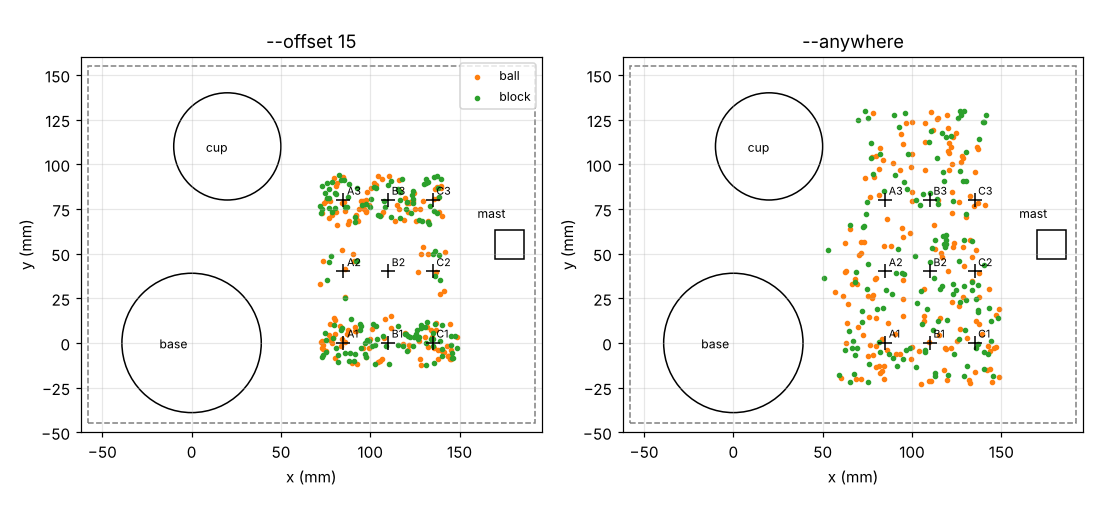
\includegraphics[width=\linewidth]{sim_layouts}
\caption{Where the simulator puts the object to pick, 300 layouts each. Left:
\texttt{--offset 15} (round the spots). Right: \texttt{--anywhere} (everywhere the arm can pick
and the camera can see). The empty strip on the right is where the open fingers would hit the
mast's foot; further toward the camera an object leaves the bottom of the picture.}
\label{fig:simlayouts}
\end{figure}

\subsection{Step 3: train on real and simulated demos together}
Export both sets into one dataset with \texttt{--with}, and give it its own name so the
real-only model stays for comparison:
\begin{cmd}
cd software\act
uv run export_act.py --with pick_ball_mujoco --out pick_ball_mix
uv run train_act.py --name pick_ball_mix --steps 20000
\end{cmd}
For GR00T, the same with \file{export_dataset.py}, then copy \file{data/lerobot/pick_ball_mix}
up and fine-tune it as in \cref{sec:cloud}:
\begin{cmd}
uv run export_dataset.py --with pick_ball_mujoco --out ..\data\lerobot\pick_ball_mix
\end{cmd}
Start with about as many simulated demos as real ones, up to twice as many (e.g.\ 150 real +
150--300 simulated). Too many simulated ones make the model better at the simulator than at the
real arm. You don't have to delete any: \texttt{--with-max N} takes only $N$ of them, spread
evenly over the whole set, and you can export several mixes under different names:
\begin{cmd}
uv run export_act.py --with pick_ball_mujoco --with-max 300 --out pick_ball_mix300
\end{cmd}

\subsection{Step 4: score models in the simulator}
\begin{cmd}
uv run ..\run_policy.py act --mujoco --trials 20 ^
    --checkpoint ..\..\outputs\act\pick_ball_mix\checkpoints\020000\pretrained_model
\end{cmd}
Twenty runs, ball and block taking turns, each on a new random layout, each stopping as soon as
an object lands in the cup. At the end it prints e.g.\ \texttt{ball: 9/10 ok (1 missed)}. Add
\texttt{--anywhere} (or \texttt{--offset 15}) to test positions off the spots: that score says
how well it copes with objects put down anywhere. Run the same command with the real-only
model's checkpoint to compare the two; GR00T works too (\texttt{run\_policy.py gr00t --mujoco
--trials 20}, with the server and SSH tunnel running). Without \texttt{--trials} it asks for
instructions like on the real arm and sets up a new layout for each.

A model saves a checkpoint every few thousand steps, and the last one isn't always the best.
\texttt{--step} picks one by its step (\texttt{--step 60k}), or scores several one after another on
the same layouts and prints a table: \texttt{run\_act.py --model pick\_ball\_mixed --step all
--mujoco --trials 20 --anywhere}. Trial~$i$ always gets the same layout, so scores from different
runs compare fairly too.

Add \texttt{--record} and the \texttt{ok} runs are saved to \file{data/raw/pick_ball_mujoco}:
this is the ``learn from its own runs'' loop of \cref{sec:selfrecord}, with the simulator
answering \texttt{keep it?}, so it can run unattended (e.g.\ \texttt{--trials 200 --record}).

\subsection{Step 5: the real test}
A simulator score is a quick way to compare models, not a promise. The model that counts is the
one that works on the real arm: run the best one there (\cref{sec:selfrecord} commands, without
\texttt{--mujoco}), with the same instructions and a few layouts on and off the spots, and
compare it with the real-only model.

\begin{note}[What the simulator gets wrong]
\begin{itemize}[leftmargin=*]
\item \textbf{Looks.} The pictures are drawn, not photographed: simpler light and surfaces, simpler
  shadows (on, as the simulated demos were recorded; a model has to be tested with the same look
  it was trained on, so \texttt{SIM\_SHADOWS=0} is only for a model trained without them), no blue servo
  bodies or cables (only the printed parts are in the model), no camera noise or blur. That's why the real demos stay in the training mix, and why step 1 matters.
\item \textbf{Servos.} SG90 dead band, gear slop and jitter aren't modelled, so the simulated
  arm moves more cleanly than the real one.
\item \textbf{Geometry.} The simulated arm is exactly where \file{config.py} says. Corrections
  for the real arm's small errors (\texttt{SPOT\_FIX} in \file{autodemo.py}) aren't used there.
\item \textbf{Objects.} The foam ball is a firm sphere with soft contacts, not real foam.
\end{itemize}
\end{note}

\section{Troubleshooting}

\begin{table}[H]
\centering\small
\begin{tabularx}{\linewidth}{@{}p{4.6cm}X@{}}
\toprule
Symptom & Fix \\
\midrule
``No Arduino found'' & Check the USB cable carries data; pass \texttt{--port COM5}. \\
Port opens but nothing moves & Supply off, no common ground, or the Serial Monitor is holding the port. Test by hand: Serial Monitor at 115200, type \texttt{90,90,90,90,125}, then \texttt{?} (\cref{sec:serial}). \\
Upload fails & Try the other bootloader (the script does both); close other programs using the port. \\
Servos twitch / Nano resets & Servo power must come from the supply; Nano GND tied to supply $-$; add the capacitor. \\
A joint moves the wrong way & \file{calibrate.py}: \texttt{test}, then \texttt{flip <joint>}. \\
Arm sags or buzzes holding pose & Normal for SG90s near their limit, mostly at the shoulder; keep the gripper light. An MG90S at the shoulder is a drop-in upgrade. \\
The drum turns instead of the arm & Fix the drum in its baseplate ring with tape or hot glue. \\
``Camera N didn't open'' & Try \texttt{--camera 0}, \texttt{1}, \texttt{2}; is the webcam plugged in (or the phone app running)? \\
A servo spins non-stop & It's a 360\textdegree{} continuous servo; swap it for a 180\textdegree{} one (\cref{sec:servotest}). \\
``can't reach that'' in teleop & The target is out of reach or the gripper would hit the plate. Move back. \\
GR00T: \texttt{GatedRepoError} & Your HF account hasn't been granted Cosmos-Reason2-2B access yet, or \texttt{HF\_TOKEN} is wrong. \\
\texttt{run\_policy}: server not reachable & Is \file{serve.sh} running and the SSH tunnel open? \\
\texttt{run\_policy}: ``policy call failed'' & One slow or failed GR00T reply; it retries. After 3 in a row it stops that run and asks again: check the SSH tunnel and \file{serve.sh}. \\
\texttt{run\_policy}: ``N limited'' & The model asked for a pose past a joint limit or into the plate, so the arm only went as far as is safe (the gripper still opened or closed as asked). A few near the grip are normal: the demos grip only about 2\,mm above the limit. Many all the time means more or better demos. \\
Policy runs but misses & More demos, more varied object positions, same camera position as in training. \\
Picks the wrong object & More demos (both objects about equally), and check the instructions saved in \file{meta.json} match what was picked. \\
\texttt{--mujoco}: ``gladLoadGL error'' or a black picture & The simulator couldn't draw: update the graphics driver. On a Linux machine without a screen it uses \texttt{MUJOCO\_GL=egl} (needs \texttt{libegl1}). \\
``20 simulated picks in a row failed'' & The simulator uses your \file{calibration.json}: check it with \file{calibrate.py} \texttt{test}, and that the gripper's open/closed angles are right. \\
``no reachable layout with \texttt{--offset}'' & The offset puts the objects out of reach or out of view; use a smaller one (15 works), or \texttt{--anywhere}. \\
Good score in the simulator, poor on the real arm & The pictures differ too much: redo the camera check (\cref{sec:sim}), and keep more real demos in the mix. \\
\file{train_act.py}: ``Output directory \dots already exists'' & An earlier model is there. Rename \file{outputs/act/pick_ball} (e.g.\ to \file{pick_ball_round1}) and run it again (\cref{sec:selfrecord}). \\
\bottomrule
\end{tabularx}
\end{table}

\section{Where everything is}

\begin{description}[leftmargin=0pt,font=\ttfamily\normalsize]
\item[cad/] \file{arm.py} (work-cell parts), \file{assembly.py} (collision and reach checks
  on the author's model), \file{sim_meshes.py} (the simulation's meshes), \file{stl/}, \file{renders/}, and the arm itself (mobiobi's files,
  CC BY-NC-SA, with \file{ATTRIBUTION.md}) in \path{stl_opensource/easy_robot_arm/}
\item[firmware/] \file{arm/arm.ino}, \file{upload.ps1}
\item[software/] \file{config.py} (geometry, calibration), \file{kinematics.py} (+ tests),
  \file{calibrate.py}, \file{teleop.py}, \file{autodemo.py}, \file{recorder.py},
  \file{export_dataset.py}, \file{policy_client.py}, \file{run_policy.py}, \file{sim.py}
  (the MuJoCo simulation) with its meshes in \file{sim_assets/}
\item[software/gr00t/] \file{gr00t_arm_config.py}, \file{setup_cloud.sh}, \file{finetune.sh}, \file{serve.sh}
\item[software/act/] \file{export_act.py}, \file{train_act.py}
\item[context.md] running notes on the project's state
\end{description}

\begin{thebibliography}{9}
\bibitem{gr00tn1} NVIDIA et al., ``GR00T N1: An Open Foundation Model for Generalist Humanoid
  Robots,'' arXiv:2503.14734, 2025.
\bibitem{isaacgr00t} NVIDIA, ``Isaac GR00T'' (code, GR00T N1.7 model, fine-tuning guides),
  \url{https://github.com/NVIDIA/Isaac-GR00T}.
\bibitem{act} T.~Z. Zhao, V.~Kumar, S.~Levine, C.~Finn, ``Learning Fine-Grained Bimanual
  Manipulation with Low-Cost Hardware,'' RSS 2023, arXiv:2304.13705.
\bibitem{easyarm} mobiobi, ``Easy Robot Arm (SG90 servos \& now steppers too),'' Printables
  model 97370, CC BY-NC-SA,
  \url{https://www.printables.com/model/97370-easy-robot-arm-sg90-servos-now-steppers-too-update}.
\bibitem{lerobot} Hugging Face, ``LeRobot,'' \url{https://github.com/huggingface/lerobot}.
\end{thebibliography}

\end{document}
